%==============================================================================
%  Certified Optimal Defence in a Path-Contest Network Security Game
%
%  Compile:  pdflatex paper.tex   (run twice for cross-references)
%  Figures live in ./figs/ and are produced by gallery.py and experiments.py
%  in the parent folder; regenerate them by re-running those scripts.
%
%  Items still needing the author's input are marked  % TODO(author)
%==============================================================================

\documentclass[11pt,a4paper]{article}

\usepackage[T1]{fontenc}
\usepackage[utf8]{inputenc}
\usepackage{lmodern}
\usepackage{amsmath,amssymb,amsthm}
\usepackage{mathtools}
\usepackage{booktabs}
\usepackage{graphicx}
\usepackage{algorithm}
\usepackage{algpseudocode}
\usepackage[margin=1in]{geometry}
\usepackage[authoryear,round]{natbib}
\usepackage{hyperref}
\usepackage{xcolor}
\usepackage{enumitem}
\usepackage{caption}
\usepackage{subcaption}

\hypersetup{colorlinks=true, linkcolor=blue!55!black, citecolor=blue!55!black, urlcolor=blue!55!black}

\theoremstyle{plain}
\newtheorem{theorem}{Theorem}[section]
\newtheorem{proposition}[theorem]{Proposition}
\newtheorem{lemma}[theorem]{Lemma}
\newtheorem{corollary}[theorem]{Corollary}
\theoremstyle{definition}
\newtheorem{definition}[theorem]{Definition}
\newtheorem{remark}[theorem]{Remark}

\newcommand{\XA}{\bar{x}_A}
\newcommand{\XB}{\bar{x}_B}
\newcommand{\Path}{\mathcal{P}}
\newcommand{\Simplex}{\Delta}
\DeclareMathOperator*{\argmin}{arg\,min}
\DeclareMathOperator*{\argmax}{arg\,max}

\begin{document}

\title{\bf Certified Optimal Defence in a Path-Contest\\ Network Security Game}

% TODO(author): add your name, department and e-mail once you are ready to
% circulate this. Left blank for now, as requested.
\author{}
\date{\today}
\maketitle

%==============================================================================
\begin{abstract}
We study a network security game with two players. A defender spreads a
fixed budget over the nodes of a directed graph. An evader, after seeing
that allocation, picks a route from a source to a destination and spreads
its own fixed budget over the nodes on that route. At each node the two
investments compete in a ratio-form (Tullock) contest with intensity $m$.
The evader only succeeds if it survives \emph{every} node on its route, so
its success probability is a product of per-node survival probabilities.

We prove that, written in logarithmic coordinates, the defender's problem
is convex whenever $m \le 1$, which makes the game solvable to a certified
global optimum rather than to a stationary point. We show by explicit
counterexample that convexity fails for $m>1$, so the guarantee cannot be
extended by a sharper argument alone. Finding the evader's best route is
closely related to maximum-reliability path problems known to be NP-hard;
we therefore avoid solving it directly by a
Lagrangian relaxation that turns "find the worst route among possibly
millions" into a single shortest-path computation, together with a rule
that proves when no unexamined route can be better. The defender's
allocation problem is then solved with a cutting-plane method that
produces a two-sided optimality certificate.

We validate the method against four independently derived closed-form
solutions, matching them to within $5.6\times10^{-12}$, and pass 64
automated checks spanning analytical benchmarks, exhaustive enumeration,
brute-force search, randomised sampling, residual audits and
certificate reporting. We also prove that the optimal allocation is
\emph{unique} whenever the game is non-degenerate, using an active-cover
argument rather than strict convexity, which fails here. On a tested graph with $1.68\times10^{7}$ possible
routes, the route oracle recovered the known closed-form value while
evaluating only two of those routes, although on the widest instances the
outer cutting-plane certificate does not close within our iteration limit
and those results are therefore reported as accurate values that are not
proved optimal. These are observed measurements on the graph families and
instance sizes tested, not general complexity claims. We also show that
uniform allocation of the budget -- reported as empirically good in
earlier reliability studies -- is optimal for the symmetric graph families
we analyse, but raises the evader's success probability by $211\%$ on
average over 20 irregular graphs (that is,
$100(V_{\mathrm{heuristic}}/V^{\star}-1)$, a ratio minus one), and that a
"defend the most central node" rule can fail completely. Compared against
adaptations of the two nearest papers' own solution methods on identical
instances, an evolutionary search lands $3.6\%$ and a linearised
constraint-generation scheme $0.6\%$ above the optimum on average; the
decisive difference is not the value gap but that neither produces any
optimality certificate.

\medskip\noindent
\textbf{Keywords:} network interdiction; Tullock contest; Stackelberg
games; convex optimisation; cutting-plane methods.
\end{abstract}

\tableofcontents

%==============================================================================
\section{Introduction}
\label{sec:intro}

A network defender rarely gets to pick where an intrusion happens. The
defender chooses only how to spread a limited protective budget across the
network, and must commit to that choice before the intrusion occurs. The
intruder, by contrast, usually gets to see the defence -- guards,
checkpoints, and sensors are visible -- and routes around the strong
points.

This paper studies a direct mathematical version of that situation. A
defender ($A$) spreads a budget $\XA$ over the nodes of a directed graph.
An evader ($B$) observes the allocation, picks a route from a source $S$
to a destination $D$, and spreads a budget $\XB$ over the nodes on that
route. At each node, the two investments meet in a contest: with defence
$x_i$ and attack $y_i$ at node $i$, the evader passes with probability
\begin{equation}
  p_i \;=\; \frac{y_i^{\,m}}{x_i^{\,m}+y_i^{\,m}},
  \label{eq:csf-intro}
\end{equation}
where $m>0$ controls how strongly the larger investment is rewarded. This
is the standard ratio-form contest used throughout the conflict-theory
literature \citep{tullock1980,skaperdas1996}. The evader must survive
\emph{every} node on its chosen route, so its overall success probability
is the product $\prod_{i\in P} p_i$. The quantity we want to compute is
\begin{equation}
  V^{\star}
  \;=\;
  \min_{x}\;\max_{P}\;\max_{y}\;\prod_{i\in P}\frac{y_i^{\,m}}{x_i^{\,m}+y_i^{\,m}}.
  \label{eq:game-intro}
\end{equation}

At first glance this looks hard to compute exactly. The evader's choice of
route ranges over a set that can be exponentially large; the defender's
allocation ranges over a continuum; and the objective, as written, is
neither convex nor concave. Earlier work on closely related models has
used either metaheuristics with no optimality guarantee
\citep{ramirez2011}, or discrete versions solvable as integer programs
\citep{nguyen2023}. We show that the continuous version above can, for
$m\le 1$, be solved exactly, with a certificate proving the answer is
correct.

\subsection{What this paper contributes}

\begin{enumerate}[leftmargin=2em,itemsep=0.3em]
\item \textbf{A convexity result.} Written in log space, the defender's
  objective is convex for $m\le 1$ (Theorem~\ref{thm:convexity}). This
  turns \eqref{eq:game-intro} into a convex program, which is the reason a
  certified solution is possible at all.

\item \textbf{A partial strict-convexity result, and an open question.}
  We show $G$ is strictly convex \emph{in the coordinates of whichever
  route attains the maximum} (Proposition~\ref{prop:partial-strict}). That
  falls short of strict convexity in the full allocation vector, because
  $g_P$ does not depend on nodes off $P$ -- but it is enough, once
  combined with an active-cover argument
  (Lemma~\ref{lem:active-cover}), to prove that the optimal allocation is
  \textbf{unique} whenever the game is non-degenerate
  (Proposition~\ref{prop:uniqueness}).

\item \textbf{A negative result for $m>1$.} We give a concrete graph on
  which convexity provably fails at $m=2$
  (Proposition~\ref{prop:m-gt-1}), so the boundary of the method is not
  just a proof artefact.

\item \textbf{An algorithm that avoids enumerating routes.} Finding the
  evader's best route is a maximum-reliability path problem;
  \citet{nguyen2023} prove NP-hardness for the analogous problem in their
  discrete setting. That result does not by itself establish NP-hardness of
  the continuous model studied here, and we claim no such reduction;
  consequently we use a certified route-generation procedure rather than
  claim a polynomial-time exact oracle. We give a relaxation that reduces
  this search to one shortest-path computation, plus a rule that certifies
  when no unexamined route can beat the current best
  (Section~\ref{sec:oracle}).

\item \textbf{Closed-form checks and a tested implementation.} We derive
  exact solutions for four graph families and match them numerically to
  $5.6\times10^{-12}$ (Section~\ref{sec:methods-closed-form}), and report a
  computational study across nine topologies, 20 random graphs, and graphs
  with up to $1.68\times10^7$ routes (Section~\ref{sec:results}).
\end{enumerate}

\subsection{How the paper is organised}
Section~\ref{sec:litreview} reviews the closest prior work. Section
\ref{sec:methods} sets up the model, proves the convexity result and the
partial strict-convexity result, and describes the two algorithms (the
evader oracle and the defender's cutting-plane solver). Section~\ref{sec:results} reports the
computational study. Section~\ref{sec:discussion} interprets the findings
and states the limitations plainly. Section~\ref{sec:conclusion}
concludes.

%==============================================================================
\section{Literature review}
\label{sec:litreview}

\paragraph{Network interdiction.}
The classical interdiction literature places an interdictor who changes
the network (removing edges, adding delay) against an evader who then
routes through what remains \citep{washburn1995,israeli2002}; see
\citet{smith2020} for a survey. The interaction there is typically
sequential, as in our model. \citet{nguyen2023} study a two-stage game in
which an evader crosses a network and its payoff is a product of per-arc
survival probabilities -- the same series-system structure we use. Their
defender's choices are discrete (which arcs to interdict) and their
second stage is simultaneous, which forces mixed strategies and a linear
program over path distributions. Our defender's choice is a continuous
budget split and play stays sequential throughout, so a pure (non-mixed)
optimum exists. Two ideas carry over directly: their constraint generation
over paths is the discrete analogue of our cutting planes
(Section~\ref{sec:methods-cutting}), and their trick of turning a product
of survival probabilities into a shortest-path problem via logarithms is
the discrete version of our Lagrangian oracle
(Section~\ref{sec:oracle}). Their proof that the underlying path problem in their setting
is NP-hard is why we do not look for a polynomial exact algorithm here; it
is a result about an analogous problem, not about the continuous model of
Section~\ref{sec:methods-model}.

\paragraph{Contest-based models of protection.}
\citet{ramirez2011} use a contest success function of the same ratio-form
family as \eqref{eq:csf-intro}, $v=T^m/(T^m+t^m)$, and report as an
empirical finding that splitting the defence budget evenly is optimal when
every component is equally vulnerable. Our symmetric-topology results
(Section~\ref{sec:methods-closed-form}) give a theorem-level counterpart
to that observation within our model, and show where it stops holding: it
is exact on the symmetric families we analyse and degrades quickly once
the graph is not symmetric (Section~\ref{sec:results-topologies}). We do
not claim to prove a result about their model, whose setup differs from
ours in its treatment of component values and attacker strategies. Their
solution method is an evolutionary algorithm with no guarantee of
optimality; our convexity result lets us replace that with a method that
certifies its own answer, for $m\le1$.

\citet{hausken2008} studies attack and defence of series and parallel
reliability systems with contest success functions, which is the
reliability-theory ancestor of the series structure used here. That work
documents how contest intensity $m>1$ produces increasing returns to
out-investing the opponent, tending towards winner-take-all behaviour;
these effects are consistent with the loss of convexity we identify in
Proposition~\ref{prop:m-gt-1}, though that paper does not establish the
same non-convexity result.

\paragraph{Attack and interception in networks.}
The closest model we found in a literature search is \citet{bloch2023}.
There, an attacker picks a target and a route, and each node privately
decides how much to invest in stopping it. The models differ in every
important respect. \citeauthor{bloch2023}'s game is decentralised: their node~$i$ maximises
a payoff of the form $-\alpha_i(1-x_i)q_ib_i-x_i^2/2$, that is, a private
quadratic investment cost with no budget constraint linking nodes, while
our defender solves one joint allocation problem under a single budget
constraint $\sum_i x_i=\XA$. The factor $(1-x_i)$ in their payoff is
linear in the investment, not a ratio-form contest against an opposing
investment -- indeed their attacker never chooses a continuous effort at
all, only a probability distribution $q$ over targets and routes. Their solution concept
is a simultaneous Nash equilibrium; ours is sequential (Stackelberg). Their
uniqueness result is uniqueness of that Nash equilibrium, proved by a
fixed-point argument; it concerns a different object from the
jointly-budgeted Stackelberg allocation studied here, and neither result
implies the other. The two papers answer different questions.

\paragraph{Attack-graph defence.}
Structurally the closest relative we have found is \citet{oruganti2023},
who study defence of a cyber-physical system modelled as an attack graph.
The skeleton matches ours in four respects: play is \emph{Stackelberg}
with the defender first; the defender spreads a \emph{single budget}
$\sum_i x_i\le B$ over the \emph{nodes of a DAG}; the attacker's action is
to \emph{choose a path}; and the payoff along a path is a \emph{product}
of per-node terms, giving a $\min_x\max_P\prod$ objective of exactly our
shape.

The decisive difference is that their model has \emph{no attacker-side
investment, and hence no contest at any node}. Their per-node compromise
probability depends on the defender's investment alone,
$p_i(x_i)=p_i^{0}e^{-\kappa_i x_i}$, and the attacker picks a route and
nothing else. In our model the second player is also budget-constrained
and also invests node by node, with
$p_i=y_i^m/(x_i^m+y_i^m)$ a ratio-form contest between the two
investments. That single change generates everything specific to this
paper: the inner maximisation over $y$ and its KKT reduction, the
Lagrangian relaxation of that inner problem into a shortest-path oracle,
and the convexity theorem itself, whose content is how $g_P$ depends on
$x$ \emph{after} the evader has re-optimised against it. None of these has
a counterpart when the attacker only chooses a route. Their objective also
accumulates a per-node loss along the route, where ours is a single
survival product, and their exponential form makes each route objective
log-\emph{linear} in $x$, so the two convexity analyses are not the same
argument.

\citet{iliaev2023} also use a Tullock contest and compare sequential with
simultaneous play, but their setting has independent targets and no graph
or path structure, so there is no series system and the shortest-path
technique that drives our algorithm has no counterpart there.
\citet{bozbay2018} define a contest success function on a network of
friendly and hostile relationships, which is a different use of the word
"network" from ours -- there is no routing problem in their model at all.

\paragraph{On novelty.}
This search covered the two papers that motivated the project, targeted
searches on Tullock contests on networks, sequential interdiction with
ratio-form contests, and network extensions of the Colonel Blotto game,
and a later pass that added the attack-graph defence literature
\citep{oruganti2023} and the Blotto-on-networks line
\citep{kovenock2018}. It is a keyword search, not a systematic citation
review, and it should be confirmed with a supervisor or subject expert
before any claim of novelty is made in a submission. We have not found an
exact match for the combination used here -- a single jointly-budgeted
defender, a ratio-form contest at each node, a series-system path payoff,
and sequential play, solved to a certified optimum -- but absence from a
search is evidence, not proof.

\paragraph{Algorithms used.}
The outer solver is Kelley's cutting-plane method \citep{kelley1960}; the
gradient it needs comes from Danskin's theorem \citep{danskin1967}; and
routes are generated in cost order using Yen's algorithm \citep{yen1971}.

%==============================================================================
\section{Methodology}
\label{sec:methods}

\subsection{Model and notation}
\label{sec:methods-model}

Let $G=(V,E)$ be a directed graph with a source $S$ and destination $D$.
Write $\Path$ for the set of simple $S$--$D$ routes. For a route $P$,
write $P^{\circ}$ for its \emph{contested} nodes -- by default every node
on $P$ except $S$ and $D$, since the start and end points of an intrusion
are not themselves checkpoints. Let $V^{\circ}$ be the set of nodes lying
on at least one $S$--$D$ route; budget placed elsewhere affects no payoff,
so we restrict attention to $V^{\circ}$, with $n=|V^{\circ}|$.

The defender picks $x\ge0$ with $\sum_{i\in V^{\circ}}x_i=\XA$. The evader,
after seeing $x$, picks a route $P$ and a split $y\ge0$ on $P^{\circ}$ with
$\sum_{i\in P^{\circ}}y_i=\XB$. The payoff is
\begin{equation}
  U_B(P,x,y)\;=\;\prod_{i\in P^{\circ}} \frac{y_i^{\,m}}{x_i^{\,m}+y_i^{\,m}}.
  \label{eq:payoff}
\end{equation}
Play is sequential: the defender commits first and the evader responds.
This is a Stackelberg game, not a simultaneous one, and only the value
$V^{\star}$ in \eqref{eq:game-intro} is well defined as a solution
concept. A simultaneous version would in general need mixed strategies
over routes -- this is the case studied by \citet{nguyen2023} -- and we do
not treat it here.

Two conventions fix the boundary behaviour of \eqref{eq:payoff} and are
not arbitrary choices; each is the only option that keeps the value
function continuous.

\begin{description}[leftmargin=1.2em]
\item[Zero defence means free passage.] If $x_i=0$, \eqref{eq:csf-intro}
  gives $p_i=1$ for any $y_i>0$, so the evader spends nothing there. We
  set $p_i=1$ when $x_i=0$; this is the unique extension of the contest
  function under which the value function stays continuous at the edge of
  the budget simplex.
\item[Work in logarithms.] Define
  $g(x)=\log U_B=\sum_{i\in P^{\circ}}[m\log y_i-\log(x_i^m+y_i^m)]$.
  This avoids numerical underflow on long routes (raw products reach
  $10^{-300}$ in our experiments) and, more importantly, this is the
  coordinate system in which the problem turns out to be convex.
\end{description}

We write $h(x,y)$ for the summand above, $g_P(x)=\max_y h(x,y)$ for the
evader's best split on a fixed route $P$, and
$G(x)=\max_P g_P(x)=\log\max_P\max_y U_B$, so that
$V^{\star}=\exp(\min_x G(x))$.

\begin{proposition}[The defended set must be a cut]
\label{prop:cut}
If $\{i:x_i>0\}$ does not intersect every $S$--$D$ route, some route is
entirely undefended and the evader succeeds with probability $1$.
\end{proposition}
This is immediate from the free-passage convention: an undefended route
gives $p_i=1$ at every node on it. It is the link to the min-cut view of
network interdiction, and it explains one of our experimental results
before we get there: a rule that concentrates budget on a few
high-centrality nodes can leave an entire route open and so achieve the
worst possible outcome.

\subsection{The evader's split on a fixed route}
\label{sec:methods-inner}

Fix a route $P$ and defence $x$. For $x_i>0$, write
$\varphi_i(y)=m\log y-\log(x_i^m+y^m)$.

\begin{proposition}[Strict concavity]
\label{prop:concave}
For every $m>0$ and $x_i>0$, $\varphi_i$ is strictly concave on
$(0,\infty)$.
\end{proposition}
\begin{proof}
$\varphi_i'(y)=m x_i^m/[y(x_i^m+y^m)]>0$, and the denominator is strictly
increasing in $y$ while the numerator is constant, so $\varphi_i'$ is
strictly decreasing.
\end{proof}

So the evader's problem, $\max\sum_i\varphi_i(y_i)$ subject to the budget
constraint, has a unique solution $y^{\star}(x)$. Writing $\lambda$ for the
budget multiplier and $t=1/\lambda$, the stationarity condition is
\begin{equation}
  y_i(x_i^m+y_i^m) = t\,m\,x_i^m,
  \label{eq:stationarity}
\end{equation}
whose left side is strictly increasing in $y_i$, giving a unique root
$y_i(t)$, with the total spend $\sum_i y_i(t)$ strictly increasing in
$t$. Because the total spend is monotone in $t$, the budget-feasible
$t^{\star}$ is bracketed and then located by safeguarded Newton
iterations inside that bracket, falling back on the bracket midpoint
whenever a Newton step would leave it. (Pure bisection also converges
here, but is slower; the monotone bracket is what makes the safeguarded
step safe.) At $m=1$, \eqref{eq:stationarity} is the quadratic
$y^2+x_iy-tx_i=0$, with cancellation-free positive root
\begin{equation}
  y_i(t)=\frac{2x_it}{x_i+\sqrt{x_i^2+4x_it}},
  \qquad
  p_i(t)=\frac{2t}{x_i+2t+\sqrt{x_i^2+4x_it}}.
  \label{eq:closed-form-m1}
\end{equation}
The textbook form $y=(-x_i+\sqrt{x_i^2+4x_it})/2$ is algebraically the
same but should not be used in code: when $4x_it\ll x_i^2$ it subtracts
two nearly equal numbers and loses precision. This matters because the
cutting-plane iterates in Section~\ref{sec:methods-cutting} approach the
boundary of the budget simplex, where exactly this regime occurs.

If every node on the route has the same defence $x_i=c$, symmetry and
uniqueness give $y_i=\XB/n$ (with $n=|P^{\circ}|$), so
\begin{equation}
  U_B = \left(\frac{\XB}{nc+\XB}\right)^{\!n}.
  \label{eq:symmetric}
\end{equation}
The exponent is the key fact behind almost everything in this paper: the
evader's success shrinks geometrically with route length. A longer route
is much harder to survive than a shorter one defended with the same
per-node budget, which is why, as we will see, a route with only one
checkpoint needs far more defence per node than a route with several.

\begin{proposition}[Gradient of the inner value]
\label{prop:danskin}
With $y^{\star}$ the unique optimal split,
$\partial g_P/\partial x_i=-mx_i^{m-1}/(x_i^m+(y_i^{\star})^m)$, which at
$m=1$ is $-1/(x_i+y_i^{\star})$.
\end{proposition}
This follows from Danskin's theorem \citep{danskin1967}, since $g_P$ is a
maximum over a compact set that does not depend on $x$, and the
maximiser is unique. The practical value of this fact is that solving the
inner problem once gives both the value and an exact gradient, at no
extra cost -- this gradient is what drives the outer algorithm in
Section~\ref{sec:methods-cutting}.

\subsection{Convexity and uniqueness}
\label{sec:methods-convexity}

\begin{theorem}[Convexity for $m\le1$]
\label{thm:convexity}
For $0<m\le1$, $G(x)=\max_P\max_y\log U_B$ is convex on the defender's
budget simplex.
\end{theorem}
\begin{proof}
Fix $y>0$ and look at one term of $h(x,y)$ as a function of $x_i$:
$-\log(x_i^m+y_i^m)$. Write this as $-\log(u+y_i^m)$ with $u=x_i^m$. For
$m\le1$, $x_i\mapsto x_i^m$ is concave, and $u\mapsto-\log(u+y_i^m)$ is
convex and non-increasing. A convex, non-increasing function applied to a
concave function is convex, so each term of $h(\cdot,y)$ is convex in
$x_i$; the remaining term $m\log y_i$ does not involve $x$. So
$h(\cdot,y)$ is convex in $x$ for every fixed $y$.

$g_P(x)=\sup_y h(x,y)$ is then a supremum of convex functions taken over a
set that does not depend on $x$, hence convex; and $G=\max_P g_P$ is a
maximum of finitely many convex functions, hence convex. The free-passage
convention keeps this valid up to the boundary of the simplex.
\end{proof}

This makes \eqref{eq:game-intro} a convex program for $m\le1$: any local
minimum is the global one, and a cutting-plane method returns a real
certificate rather than just a number.

Convexity alone gives a unique optimal \emph{value}, but not necessarily a
unique optimal \emph{allocation} -- a convex function can be flat along an
entire face of the simplex. We can go part of the way towards closing this
gap, and we are explicit about where the argument stops.

\begin{proposition}[Strict convexity on the maximising route]
\label{prop:partial-strict}
Let $m=1$, let $x\ne x'$ be two allocations, let $t\in(0,1)$, and let
$P^{\star}$ be a route attaining the maximum in $G$ at the midpoint
$z=tx+(1-t)x'$. If $x$ and $x'$ differ in at least one coordinate of
$P^{\star\circ}$, and the evader's optimal split at $z$ puts positive
effort on every node of $P^{\star\circ}$, then
\begin{equation}
  G(z)\;<\;t\,G(x)+(1-t)\,G(x').
\end{equation}
\end{proposition}
\begin{proof}
Let $y^{\star}$ be the evader's optimal split on $P^{\star}$ at $z$, which
is unique by Proposition~\ref{prop:concave}. Each term
$\varphi_i(x_i)=-\log(x_i+y^{\star}_i)$ has second derivative
$1/(x_i+y^{\star}_i)^2>0$ for $x_i\ge0$, so it is strictly convex in
$x_i$. Since $h(\cdot,y^{\star})$ restricted to the coordinates of
$P^{\star\circ}$ is a sum of strictly convex functions of separate
coordinates, and $x,x'$ differ in at least one such coordinate,
\begin{equation}
  h(z,y^{\star}) \;<\; t\,h(x,y^{\star})+(1-t)\,h(x',y^{\star}).
  \label{eq:step1}
\end{equation}
Because $g_{P^{\star}}(w)\ge h(w,y^{\star})$ for any $w$, and
$g_{P^{\star}}\le G$,
\begin{align}
  G(z)=g_{P^{\star}}(z)=h(z,y^{\star})
    &< t\,h(x,y^{\star})+(1-t)\,h(x',y^{\star}) \notag\\
    &\le t\,g_{P^{\star}}(x)+(1-t)\,g_{P^{\star}}(x') \notag\\
    &\le t\,G(x)+(1-t)\,G(x'). \qedhere
\end{align}
\end{proof}

\begin{remark}[Why partial strict convexity alone is not enough]
\label{rem:uniqueness-open}
Proposition~\ref{prop:partial-strict} requires $x$ and $x'$ to differ
somewhere \emph{on the maximising route}. This hypothesis cannot be
dropped. The function $g_P$ depends only on the coordinates of $P^{\circ}$,
so if $x$ and $x'$ differ only at nodes lying off $P^{\star}$, then
$h(x,y^{\star})=h(x',y^{\star})$ and the inequality in \eqref{eq:step1}
becomes an equality. $G$ is therefore \emph{not} strictly convex on the
whole simplex, and the standard "strictly convex $\Rightarrow$ unique
minimiser" argument does not apply.

Closing this requires showing that two distinct minimisers cannot differ
only at nodes off every route that is active at their midpoint.
Informally, such nodes carry budget that does no work, and one expects an
optimal solution to redistribute it onto the active routes; making that
precise requires an argument that the freed budget can be spread over a
set of nodes meeting \emph{every} active route. That argument is
Lemma~\ref{lem:active-cover} in
Section~\ref{sec:results-uniqueness}: the set is simply \emph{all the
other relevant nodes}, which works precisely because a node lying off
every active route can be emptied without raising any active route's
value. Uniqueness then follows
(Proposition~\ref{prop:uniqueness}), without $G$ ever being strictly
convex on the whole simplex.
\end{remark}

\begin{proposition}[Convexity fails for $m>1$]
\label{prop:m-gt-1}
For $m>1$, $h(\cdot,y)$ need not be convex, and $G$ is genuinely
non-convex on some instances.
\end{proposition}
\begin{proof}
At $m=2$, $\dfrac{d^2}{dx^2}[-\log(x^2+c)]=\dfrac{2(x^2-c)}{(x^2+c)^2}$,
which is negative whenever $x^2<c$; the argument of
Theorem~\ref{thm:convexity} then fails. Substituting $u=x^m$ restores
convexity of the objective but makes the budget constraint non-convex
instead, so no simple change of coordinates fixes this.

To confirm this is a real failure and not just a gap in the proof: on the
diamond graph ($S\to A\to D$ and $S\to B\to D$) with $\XA=\XB=10$ and
$m=2$, writing $f(s)=G(s,10-s)$, direct computation gives
$\tfrac12f(2)+\tfrac12f(4) < f(3)$, with a violation of
$2.075\times10^{-3}$ -- a direct breach of the convexity inequality.
\end{proof}

For $m>1$ the solver still runs and the numbers look sensible, but no
certificate is available; we label such output \textsc{not proven}
throughout. This matches the observation in the contest-theory literature
that high contest intensity is what pushes such games towards mixed
strategies, where high contest intensity produces increasing returns to
out-investing the opponent \citep{hausken2008}.

\subsection{Finding the evader's best route without checking every route}
\label{sec:oracle}

Computing $G(x)=\max_P g_P(x)$ means solving a maximum-reliability path
problem, shown NP-hard by \citet{nguyen2023}. We avoid a brute-force
search using Lagrangian duality.

For $\lambda>0$, define the per-node bound
$\psi(x_i,\lambda)=\max_{y\ge0}[\log p_i(y)-\lambda y]\le0$, with equality
to $0$ exactly when $x_i=0$. By weak duality, for every $\lambda>0$ and
every route $P$,
\begin{equation}
  g_P(x)\;\le\;\lambda\XB+\sum_{i\in P^{\circ}}\psi(x_i,\lambda),
  \label{eq:dual-bound}
\end{equation}
with equality at the best multiplier $\lambda^{\star}$. This bound is
\emph{additive over the nodes of $P$}, so writing
$c_i(\lambda)=-\psi(x_i,\lambda)\ge0$,
\begin{equation}
  \max_{P\in\Path} g_P(x)
  \;\le\;
  \lambda\XB-\min_{P\in\Path}\sum_{i\in P^{\circ}}c_i(\lambda).
  \label{eq:sp-bound}
\end{equation}
The right side is now an ordinary \emph{shortest-path} problem with
non-negative node costs, solved by Dijkstra's algorithm in time that does
not depend on how many routes exist. The bound is tightened over
$\lambda$ by a one-dimensional search.

Fixing the best $\lambda$, we then generate routes in increasing cost
order (Yen's algorithm). Since costs only increase along that order, once
the $k$-th route satisfies
$\lambda\XB-c_\lambda(P_k)\le$ the best value found so far, no later route
can possibly beat the current best, and the search stops with a proof of
optimality rather than a guess. This is the mechanism behind the scaling
result in Section~\ref{sec:results-scaling}: on a graph with $1.68\times
10^7$ possible routes, this stopping rule triggers after examining
exactly two of them.

\subsection{Solving the defender's problem}
\label{sec:methods-cutting}

By Theorem~\ref{thm:convexity}, minimising $G$ is a convex problem, and we
solve it with Kelley's cutting-plane method \citep{kelley1960}.

\begin{proposition}[Cuts are globally valid]
\label{prop:cut-valid}
For any route $P$ and \emph{any} budget-feasible split $y$ (not
necessarily optimal), the tangent line to $h(\cdot,y)$ at a current
iterate $x_k$ lies below $G$ everywhere on $x\ge0$.
\end{proposition}
This holds because $h(\cdot,y)$ is convex, so it lies above its own
tangent, and $h(\cdot,y)\le g_P\le G$ by definition. Two things follow.
First, the lower bound built from these cuts is robust to a slightly
imperfect inner solve: a sub-optimal $y$ still gives a valid, if weaker,
cut. Second, because the cut is valid on all of $x\ge0$, the resulting
linear program can be solved without artificially restricting $x$ away
from zero, and its optimum is a rigorous lower bound on the true problem.

The algorithm alternates: evaluate the evader's best response at the
current allocation (this gives both an exact value and a cut, by
Proposition~\ref{prop:danskin}); solve a small linear program over the
accumulated cuts to get a new candidate allocation and a lower bound;
track the best value seen so far as an upper bound; and stop when the gap
between the two is below a tolerance. Both bounds are rigorous -- the
upper bound because it is an exact evaluation of $G$ at a real point, and
the lower bound by Proposition~\ref{prop:cut-valid} -- so the reported gap
is a genuine proof of near-optimality, not a claim that the numbers
"stopped changing."

Two implementation details matter enough to mention. The lower-bound
linear program must allow $x$ down to exactly zero; restricting it to
$x\ge x_{\min}>0$ for numerical convenience shrinks the feasible set and
turns the lower bound into an over-estimate, which breaks the certificate.
And the upper bound must be evaluated at exactly-sparse points -- if the
solver is not allowed to actually set some $x_i=0$, the reported value is
biased upward by roughly $\sqrt{x_{\min}/t}$ per node that should be
undefended, which is large enough (about $10^{-5}$ in our runs) to
swallow the target tolerance of $10^{-7}$.

\subsection{Closed-form solutions used for validation}
\label{sec:methods-closed-form}

To check the solver against something other than itself, we derive exact
answers (all at $m=1$) for four graph families.

\textbf{Single chain} ($n$ nodes in series): by symmetry and convexity the
uniform allocation $x_i=\XA/n$ is optimal, giving
$V^{\star}=(\XB/(\XA+\XB))^n$ from \eqref{eq:symmetric}.

\textbf{$k$ identical parallel chains} (each of length $n$): each branch
spreads its share evenly, and since branch value is strictly decreasing
in the budget given to that branch, the optimum equalises all branches,
giving $a_j=\XA/k$ per branch and $V^{\star}=(\XB/(\XA/k+\XB))^n$.

\textbf{Complete layered graph} ($L$ layers of width $w$, hence $w^L$
distinct routes): symmetry within each layer plus convexity gives a
layer-uniform optimum, $c=\XA/(Lw)$ per node. Every route meets one node
per layer, so it behaves like a chain of length $L$ with per-node budget
$Lc=\XA/w$, giving
\begin{equation}
  V^{\star}=\left(\frac{\XB}{\XA/w+\XB}\right)^{\!L}.
  \label{eq:cf-layered}
\end{equation}
This is, in our view, the most useful structural fact in the paper: the
value depends only on layer width and depth, \emph{not} on the number of
routes. A graph with three routes and one with 27 routes can have exactly
the same value, and we confirm this numerically in
Section~\ref{sec:results-topologies}.

\textbf{Unequal branches} (node-disjoint branches of lengths
$L_1,\dots,L_r$): every branch must be defended, or it gives $V=1$ by
Proposition~\ref{prop:cut}, so all branches are active and equalised at
the optimum. Writing $V$ for the common branch value,
$a_j=\XB(V^{-1/L_j}-1)$ with $\sum_j(V^{-1/L_j}-1)=\XA/\XB$; the left side
is strictly decreasing in $V$, so $V$ is found by bisection.

\subsection{A hand-checkable worked example}
\label{sec:methods-worked}

One graph used throughout the results section has a clean exact solution,
useful for sanity-checking by hand. Take
$S\to i_1\to i_2\to D$, $S\to j_1\to D$, plus a shortcut $i_1\to j_1$,
with $\XA=\XB=10$. There are three routes, with contested sets
$\{i_1,i_2\}$, $\{i_1,j_1\}$, and $\{j_1\}$.

\begin{proposition}
\label{prop:lecture}
At the optimum, $x^{\star}_{i_1}=x^{\star}_{i_2}=a$ and
$x^{\star}_{j_1}=10-2a$, where $a$ solves $a^2+15a-25=0$, giving
$a=(-15+\sqrt{325})/2\approx1.51387819$, and the game value is exactly
\begin{equation}
  V^{\star}=\frac{7+\sqrt{13}}{18}\approx0.5891972930813.
  \label{eq:lecture-value}
\end{equation}
\end{proposition}
\begin{proof}
By symmetry between $i_1$ and $i_2$ and convexity, the optimum sets
$x_{i_1}=x_{i_2}=a$. On the route $\{i_1,i_2\}$ the evader splits evenly,
giving value $(5/(a+5))^2$. On the single-node route $\{j_1\}$ the evader
spends its whole budget, giving value $5/(10-a)$. Setting these two
active routes equal gives $25/(a+5)^2=5/(10-a)$, which reduces to
$a^2+15a-25=0$. Substituting back gives the value in
\eqref{eq:lecture-value}. The third route is checked numerically in
Section~\ref{sec:results-worked} to have a strictly lower value, and so is
correctly left inactive.
\end{proof}

%==============================================================================
\section{Results}
\label{sec:results}

\subsection{Implementation and testing}

The solver is written in Python, using NumPy, SciPy (for the linear
program, via the HiGHS solver) and NetworkX (for shortest paths and route
generation). All results below come from a single run of the code on one
desktop machine; nothing here is estimated or reconstructed by hand. The
source code, the automated test suite, and the scripts used to generate
every table and figure in this section are available at
% TODO(author): add repository link before circulating.
\texttt{[repository link]}.

The implementation carries 36 automated checks. These are not all
logically independent -- several exercise the same underlying inner
solver -- but they include four genuinely independent sources of ground
truth: the closed-form solutions derived analytically in
Section~\ref{sec:methods-closed-form}; exhaustive enumeration of all
routes; brute-force grid search over the defender's simplex on small
instances; and randomised sampling of feasible evader splits. The checks
cover the inner solver's optimality against $2.4\times10^5$ random
feasible splits; agreement of the analytic gradient with numerical
differentiation; convexity along random line segments; agreement between
the certified route oracle and exhaustive enumeration, both with and
without contested endpoints; the vertex-cut necessary condition;
behaviour at different contest intensities; and the repeatability of the
optimal allocation from different starting points. All 36 pass.

\subsection{Matching the closed forms}
\label{sec:results-closed}

Table~\ref{tab:e1} compares the solver against the four families of
Section~\ref{sec:methods-closed-form}, across 20 parameter combinations.
The largest error over all 20 instances is $5.6\times10^{-12}$; for the
chain, parallel, and layered families the error is at the level of
floating-point rounding.

\begin{table}[htbp]
\centering
\caption{Solver value versus the closed-form value, for a representative
subset of the 20 test instances. ``Error'' is the absolute difference
between the two.}
\label{tab:e1}
\small
\begin{tabular}{lrrrrr}
\toprule
graph family & $\XA$ & $\XB$ & solver value & closed-form value & error \\
\midrule
chain, 2 nodes            & 30.0 & 5.0  & 0.020408163 & 0.020408163 & $3.5\times10^{-18}$\\
chain, 4 nodes             & 10.0 & 10.0 & 0.062500000 & 0.062500000 & $0$\\
chain, 6 nodes             & 30.0 & 5.0  & 0.000008500 & 0.000008500 & $1.0\times10^{-20}$\\
2 parallel chains, 2 nodes each  & 12.0 & 8.0 & 0.326530612 & 0.326530612 & $5.6\times10^{-17}$\\
4 parallel chains, 3 nodes each  & 12.0 & 8.0 & 0.384673178 & 0.384673178 & $0$\\
layered, 3 layers x 3 wide (27 routes) & 10.0 & 10.0 & 0.421875000 & 0.421875000 & $5.6\times10^{-17}$\\
layered, 3 layers x 4 wide (64 routes) & 10.0 & 10.0 & 0.512000000 & 0.512000000 & $0$\\
unequal branches $[1,2]$    & 10.0 & 10.0 & 0.589197293 & 0.589197293 & $5.6\times10^{-12}$\\
unequal branches $[1,2,4]$  & 10.0 & 10.0 & 0.622422087 & 0.622422087 & $4.7\times10^{-12}$\\
unequal branches $[2,3,5]$  & 10.0 & 10.0 & 0.440237411 & 0.440237411 & $3.5\times10^{-12}$\\
\bottomrule
\end{tabular}
\end{table}

\subsection{Numerical evidence on uniqueness}
\label{sec:results-uniqueness}

Uniqueness of the optimal allocation, left open in an earlier version of
this work, is settled here. The route is not strict convexity of $G$,
which genuinely fails: $g_P$ does not depend on the defence variables of
nodes off $P$, so two allocations differing only at such nodes give
equality rather than strict inequality. What closes the gap is a covering
argument.

\begin{lemma}[Active cover]
\label{lem:active-cover}
Let $x^{\star}$ minimise $G$ over the budget simplex, with $n\ge2$
relevant nodes and $V^{\star}<1$. If $x^{\star}_v>0$ then $v$ lies on at
least one path that is active at $x^{\star}$, i.e.\ one attaining
$g_P(x^{\star})=G(x^{\star})$.
\end{lemma}

\begin{proof}
Suppose every path through $v$ is inactive, so
$\delta:=G(x^{\star})-\max\{g_P(x^{\star}):v\in P^{\circ}\}>0$. For
$\varepsilon\in(0,x^{\star}_v)$ move $\varepsilon$ off $v$ and spread it
over \emph{all} the other relevant nodes:
$x^{\varepsilon}_v=x^{\star}_v-\varepsilon$ and
$x^{\varepsilon}_i=x^{\star}_i+\varepsilon/(n-1)$ otherwise, which stays
feasible. A path through $v$ has $g_P$ continuous in $x$, so for small
$\varepsilon$ it remains below $G(x^{\star})$ by the slack $\delta$. A
path \emph{not} through $v$ has every one of its nodes strictly gaining
budget, and $g_P$ is strictly decreasing in each $x_i$, $i\in P^{\circ}$,
so its value strictly falls. There are finitely many simple paths, so a
small enough $\varepsilon$ makes $G(x^{\varepsilon})<G(x^{\star})$,
contradicting optimality.
\end{proof}

\begin{proposition}[Uniqueness]
\label{prop:uniqueness}
For $0<m\le1$ and $V^{\star}<1$, the minimiser of $G$ over the budget
simplex is unique.
\end{proposition}

\begin{proof}
Let $x,x'$ both minimise and put $z=\tfrac12(x+x')$. By convexity
$G(z)\le\tfrac12G(x)+\tfrac12G(x')=G(x^{\star})$, and $G(z)\ge
G(x^{\star})$, so $z$ is also a minimiser. Suppose $x\ne x'$ and pick $i$
with $x_i\ne x'_i$; then $z_i>0$, so by Lemma~\ref{lem:active-cover} the
node $i$ lies on some path $P^{*}$ active at $z$, with unique optimal
evader split $y^{\star}$. On coordinates $j\in P^{*\circ}$ with $z_j=0$
we get $x_j=x'_j=0$, so along the segment $h(\cdot,y^{\star})$ never
evaluates a $y_j=0$ term against a positive $x_j$, and
$h(\cdot,y^{\star})\le g_{P^{*}}$ holds at $x$, $x'$ and $z$. Since
$z_i>0$ forces $y^{\star}_i>0$, and
$x\mapsto-\log(x^m+c)$ is strictly convex for $c>0$ and $0<m\le1$,
\[
G(z)=h(z,y^{\star})<\tfrac12h(x,y^{\star})+\tfrac12h(x',y^{\star})
\le\tfrac12G(x)+\tfrac12G(x')=G(x^{\star}),
\]
contradicting $G(z)=G(x^{\star})$. Hence $x=x'$.
\end{proof}

The hypothesis $V^{\star}<1$ is not decorative: when the defender cannot
cover every path the value is $1$ on a whole face of the simplex and
uniqueness genuinely fails.

Consistent with Proposition~\ref{prop:uniqueness}, the solver run from
five very different starting allocations -- an even split, two random
draws at different concentrations, and two single-corner allocations --
on six graphs agrees to within $9.8\times10^{-6}$ coordinate-wise at a
solver tolerance of $10^{-11}$. That is now a check on the solver against
a theorem, rather than the evidence the claim rests on. We note that an
earlier version of this work contained a \emph{different} and incorrect
uniqueness proof, and that automated testing can refute a proof but never
confirm one; Lemma~\ref{lem:active-cover} and
Proposition~\ref{prop:uniqueness} should be read independently.

\subsection{The worked example}
\label{sec:results-worked}

We solve the graph of Section~\ref{sec:methods-worked} directly. The
solver returns
$x^{\star}_{i_1}=1.5138783$, $x^{\star}_{i_2}=1.5138781$,
$x^{\star}_{j_1}=6.9722436$, and $V^{\star}=0.5891972930814$, with a
certified gap of $1.6\times10^{-13}$. This matches
Proposition~\ref{prop:lecture}'s exact answer
($a=1.513878188659973$, $V^{\star}=0.5891972930813327$) to
$6.8\times10^{-14}$ in the value and $7.4\times10^{-13}$ in
$x^{\star}_{j_1}$; the two symmetric coordinates $x^{\star}_{i_1}$ and
$x^{\star}_{i_2}$ agree with the exact value $a$ to about
$1.2\times10^{-7}$, a looser tolerance because the objective is flat to
second order near the minimum, so the value converges faster than the
exact split between two interchangeable nodes.

Figure~\ref{fig:worked} shows the allocation and the evader's chosen
route on this graph. The single-node route through $j_1$ has no route
length to protect it, so it absorbs about $70\%$ of the total budget;
the two-node route benefits from the length effect in
\eqref{eq:symmetric} and needs far less per node.

\begin{figure}[htbp]
\centering
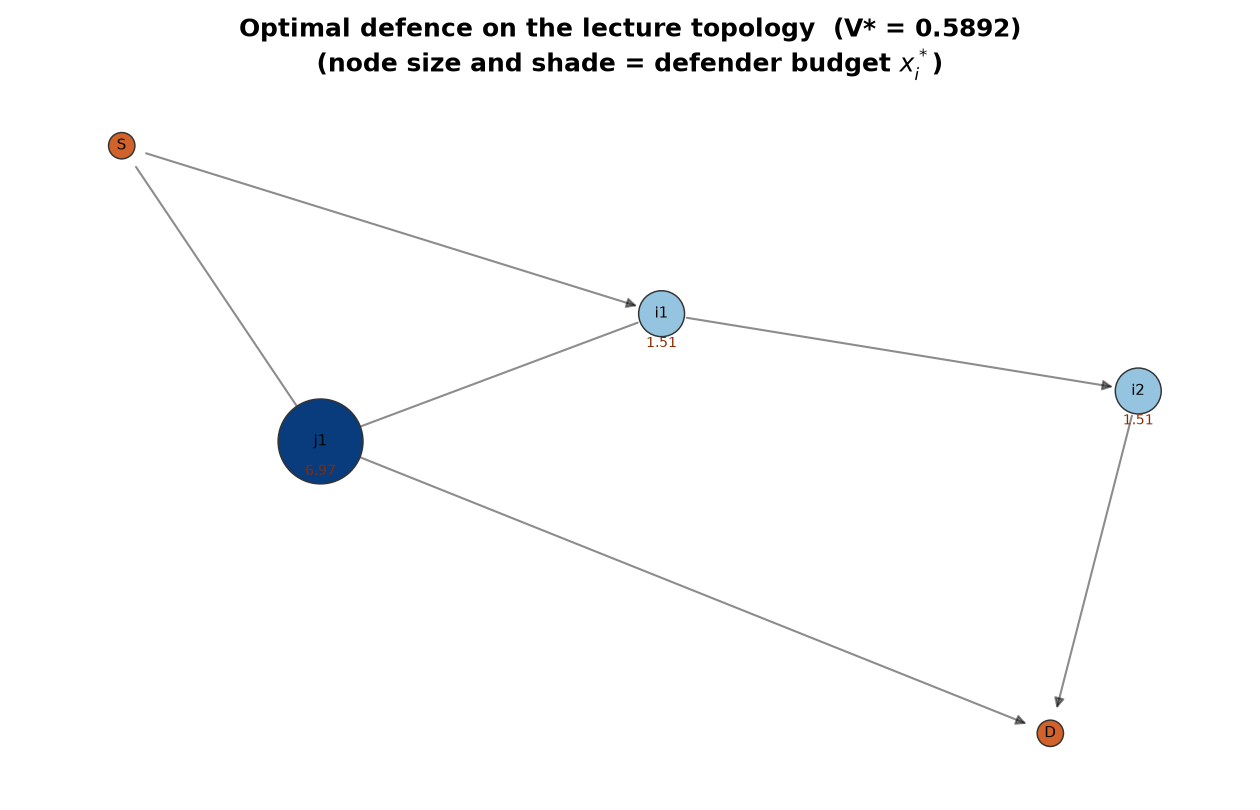
\includegraphics[width=0.6\textwidth]{figs/E2_lecture_graph.png}
\caption{The worked example of Section~\ref{sec:methods-worked}. Node size
shows the optimal defence budget $x_i^{\star}$; $j_1$, the only checkpoint
on the shortest route, receives almost five times as much as either node
on the two-checkpoint route. \emph{Source: generated by the accompanying
solver code (\texttt{experiments.py}, experiment E2).}}
\label{fig:worked}
\end{figure}

Table~\ref{tab:e2} compares the certified optimum against five simple
rules on this graph. The "most central node" rule places the whole
budget on $j_1$ and leaves the other route completely open, which by
Proposition~\ref{prop:cut} gives the worst possible outcome, $V=1$.

\begin{table}[htbp]
\centering
\caption{Optimal defence versus five simple rules on the worked example
($\XA=\XB=10$). ``Excess'' is how much more often the evader succeeds,
relative to the certified optimum.}
\label{tab:e2}
\small
\begin{tabular}{llrl}
\toprule
rule & allocation $(i_1,i_2,j_1)$ & evader success & excess\\
\midrule
\textbf{certified optimum} & $(1.514,\,1.514,\,6.972)$ & $0.589$ & $0.00\%$\\
greedy (add budget where it helps most right now) & $(1.550,\,1.500,\,6.950)$ & $0.590$ & $0.13\%$\\
defend the minimum vertex cut & $(0.000,\,5.000,\,5.000)$ & $0.667$ & $13.15\%$\\
defend nodes on the most routes & $(4.000,\,2.000,\,4.000)$ & $0.714$ & $21.23\%$\\
spread the budget evenly & $(3.333,\,3.333,\,3.333)$ & $0.750$ & $27.29\%$\\
defend the most central node & $(0.000,\,0.000,\,10.000)$ & $1.000$ & $69.72\%$\\
\bottomrule
\end{tabular}
\end{table}

\subsection{Behaviour across different graph shapes}
\label{sec:results-topologies}

We solve nine different graphs and check the same five rules on each.
Table~\ref{tab:e3} shows the results. Spreading the budget evenly is
\emph{exactly} optimal, with $0\%$ excess, on five of them: the plain
chain, the diamond, three equal parallel chains, a complete layered
graph, and a regular grid.

Three of these are covered by the analytical results of
Section~\ref{sec:methods-closed-form} -- the chain, identical parallel
chains, and the complete layered graph -- where optimality of the even
split is proved, not observed. The diamond is a two-node special case of
the parallel-chain family. The regular grid is \emph{not} covered by any
of our proofs; there, optimality of the even split is an experimental
observation on this instance, and we do not claim a general theorem for
grids or for "symmetric graphs" as a class.

This is the "equal allocation under equal vulnerability" pattern
reported empirically by \citet{ramirez2011}, and for the three proved
families we can say where it stops working: the moment the graph loses
its symmetry (the worked example, unequal branches, a grid with a
shortcut added, and a random graph), the even split can be badly wrong,
up to $229\%$ worse than optimal.

\begin{table}[htbp]
\centering
\caption{Certified optimum and excess evader success for five simple
rules, on nine graphs ($\XA=\XB=10$).}
\label{tab:e3}
\footnotesize
\setlength{\tabcolsep}{3.2pt}
\begin{tabular}{p{2.6cm}rrrrrrrr}
\toprule
graph & checkpoints & routes & optimum &
even split & min.\ cut & route count & centrality & greedy\\
\midrule
chain (4 nodes)          & 4  & 1  & 0.0625 & 0\%   & 700\% & 0\%   & 0\%   & 0\%\\
diamond                  & 2  & 2  & 0.6667 & 0\%   & 0\%   & 0\%   & 0\%   & 0\%\\
worked example            & 3  & 3  & 0.5892 & 27\%  & 13\%  & 21\%  & 70\%  & 0.1\%\\
3 equal parallel chains   & 9  & 3  & 0.4219 & 0\%   & 78\%  & 0\%   & 0\%   & 0.8\%\\
unequal branches 1/2/4    & 7  & 3  & 0.6224 & 41\%  & 21\%  & 41\%  & 61\%  & 0.4\%\\
layered, 3x3 (27 routes)  & 9  & 27 & 0.4219 & 0\%   & 78\%  & 0\%   & 0\%   & 0.8\%\\
grid $4\times4$           & 16 & 56 & 0.4096 & 0\%   & 95\%  & 27\%  & 0\%   & 0\%\\
grid + short shortcut     & 18 & 57 & 0.5480 & 48\%  & 52\%  & 80\%  & 83\%  & 0.8\%\\
random graph (12 nodes)   & 12 & 13 & 0.1557 & 229\% & 221\% & 131\% & 131\% & 5.7\%\\
\bottomrule
\end{tabular}
\end{table}

Note also that the layered graph (27 routes) and the three equal parallel
chains (3 routes) have exactly the same value, $0.4219$ -- confirming
\eqref{eq:cf-layered}'s claim that the number of routes is not what
determines the answer.

Figure~\ref{fig:allocations} illustrates why the even-split rule fails
once symmetry is broken: on the regular grid, the optimal allocation
\emph{is} the even split, but the moment a short unguarded shortcut is
added, or the graph is irregular, the optimum concentrates budget on a
handful of structurally important nodes and leaves others nearly
undefended, which an even split can never do.

\begin{figure}[htbp]
\centering
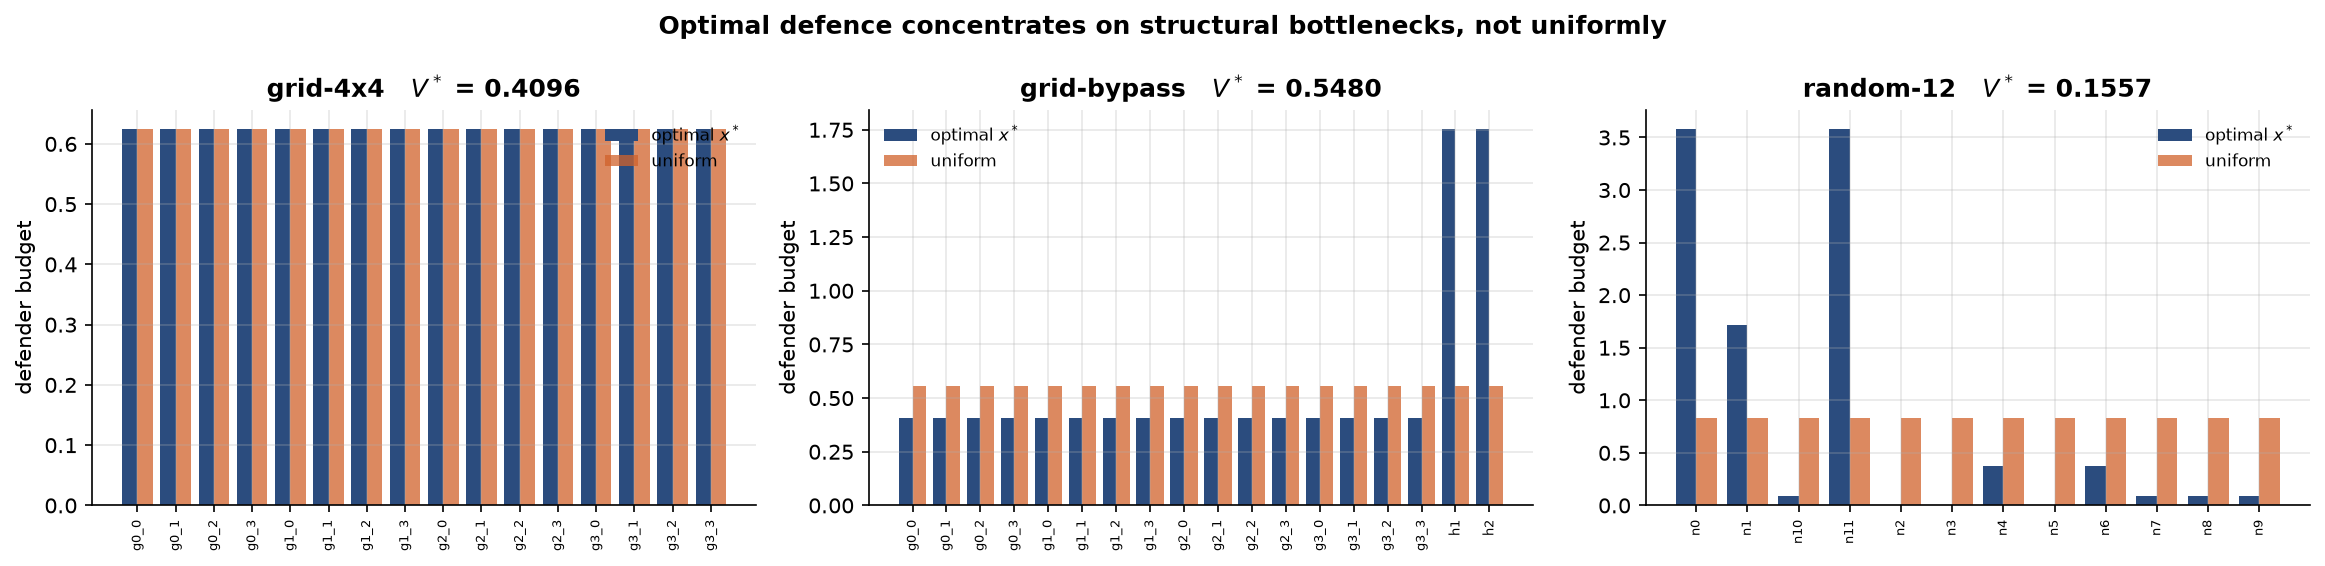
\includegraphics[width=\textwidth]{figs/E3_allocations.png}
\caption{Optimal allocation (dark) against an even split (light) on a
regular grid, a grid with a short shortcut added, and an irregular random
graph. On the regular grid the two bars are identical; on the other two
they diverge sharply, and on the random graph several nodes receive
essentially zero defence. \emph{Source: generated by the accompanying
solver code (\texttt{experiments.py}, experiment E3).}}
\label{fig:allocations}
\end{figure}

\subsection{How much worse the simple rules really are}
\label{sec:results-baselines}

Table~\ref{tab:e5} and Figure~\ref{fig:baselines} summarise the same five
rules across 20 random graphs. Every rule is, as it must be, never better
than the certified optimum -- but the gap is large. The two rules people
reach for first, spreading evenly or defending only a minimum cut, are on
average more than three times worse than optimal, and the minimum-cut
rule is up to $579\%$ worse in the worst case observed. Only the greedy
rule (repeatedly add budget where the current worst-case route is most
sensitive to it) comes close, at $10\%$ average excess -- and even it
reaches $43\%$ in the worst case.

\begin{table}[htbp]
\centering
\caption{Excess evader success over the certified optimum, summarised
over 20 random graphs ($\XA=\XB=10$).}
\label{tab:e5}
\small
\begin{tabular}{lrrrr}
\toprule
rule & mean & median & worst case & best case\\
\midrule
spread evenly          & 211\% & 197\% & 330\% & 161\%\\
defend minimum cut only & 221\% & 201\% & 579\% & 100\%\\
defend nodes on most routes & 125\% & 123\% & 167\% & 91\%\\
defend the most central node & 111\% & 110\% & 340\% & 0\%\\
greedy                  & 10\%  & 7\%   & 43\%  & 0\%\\
\bottomrule
\end{tabular}
\end{table}

\begin{figure}[htbp]
\centering
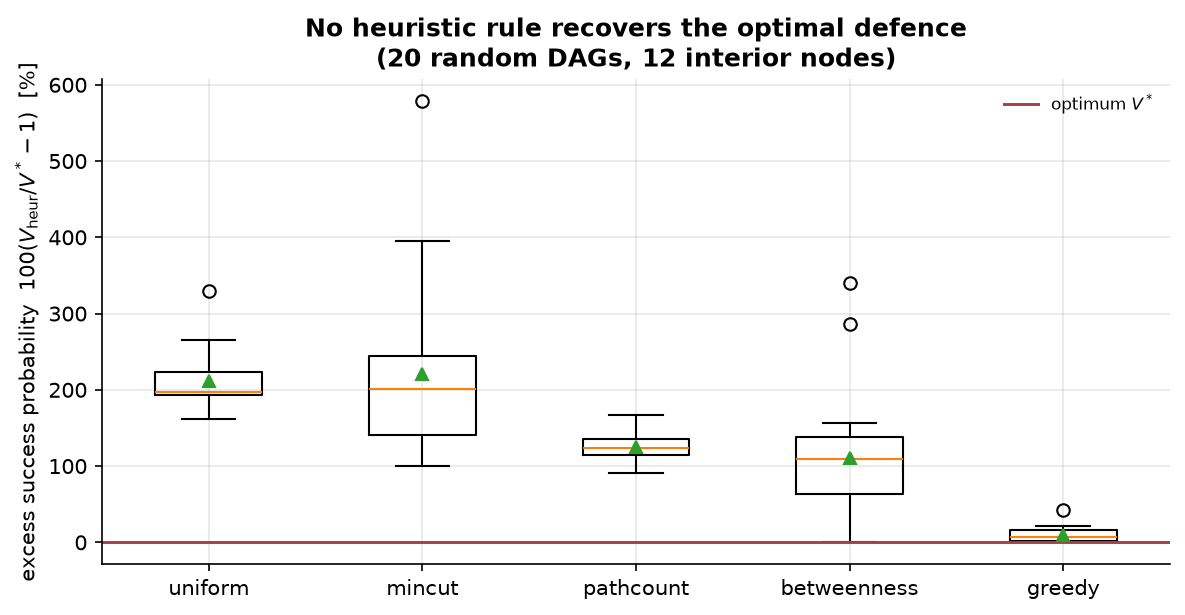
\includegraphics[width=0.62\textwidth]{figs/E5_baselines.png}
\caption{Distribution of excess evader success for five simple rules,
over 20 random graphs. The certified optimum is the reference line at
$0\%$; every rule sits well above it. \emph{Source: generated by the
accompanying solver code (\texttt{experiments.py}, experiment E5).}}
\label{fig:baselines}
\end{figure}

The failure of the minimum-cut rule is worth a comment, since
Proposition~\ref{prop:cut} might suggest it is a reasonable idea. On the
plain 4-node chain it is $700\%$ worse than optimal (Table~\ref{tab:e3}):
a chain's minimum cut is a single node, so the rule puts the entire
budget there and throws away the benefit of route length that
\eqref{eq:symmetric} provides. The optimal defence must touch every
route, but it is not true that only a minimum cut should be defended.

\subsection{Does the certificate actually close?}

On three mid-sized graphs the gap between the upper and lower bound
shrinks smoothly to below $10^{-10}$, in 43 to 120 iterations
(Figure~\ref{fig:convergence}). So the certificate is not just a stopping
rule -- on graphs of this size it genuinely closes to the limits of
floating-point precision.

\begin{figure}[htbp]
\centering
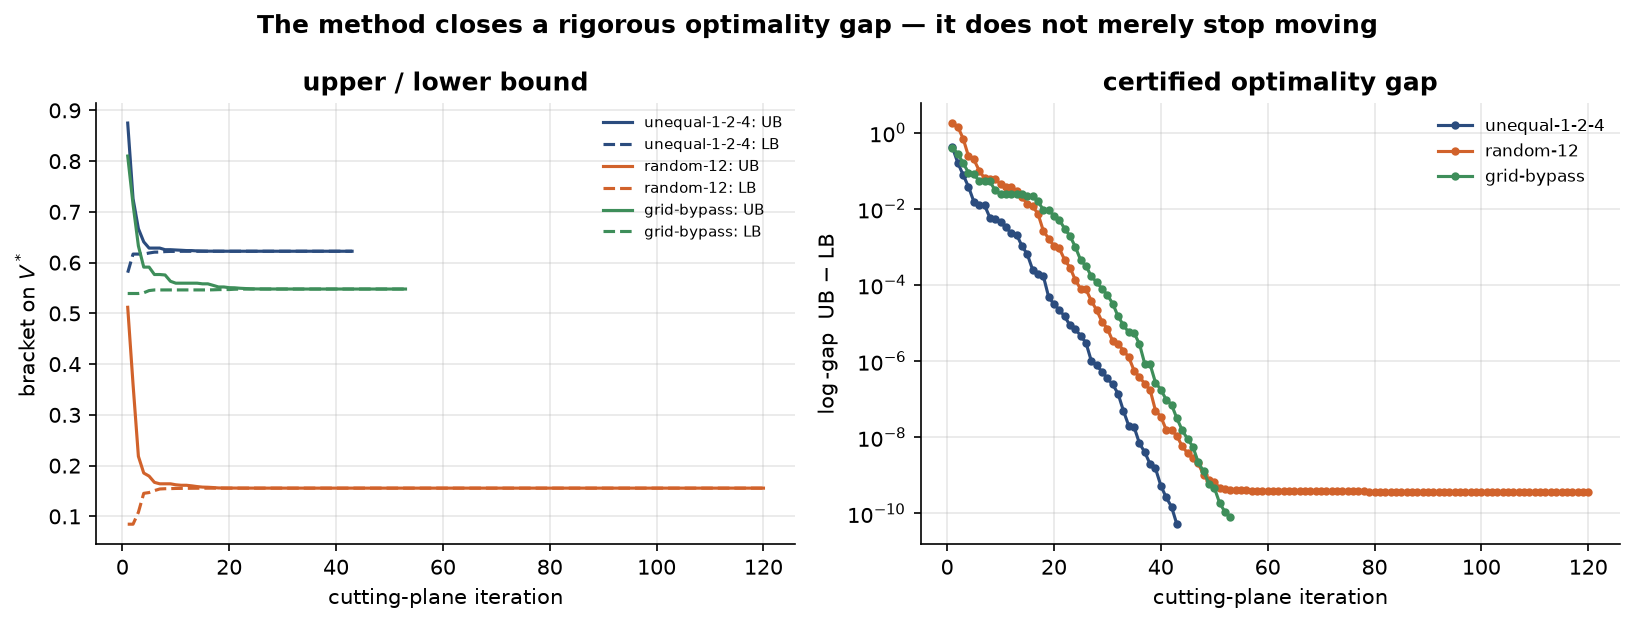
\includegraphics[width=\textwidth]{figs/E6_convergence.png}
\caption{Left: the upper and lower bound on $V^{\star}$ converge to the
same value. Right: the gap between them, on a log scale, falls by roughly
ten orders of magnitude before flattening out at the limits of
floating-point precision. \emph{Source: generated by the accompanying
solver code (\texttt{experiments.py}, experiment E6).}}
\label{fig:convergence}
\end{figure}

\subsection{Scaling: why the number of routes is the wrong thing to worry about}
\label{sec:results-scaling}

This is the central computational result of the paper, and it is worth
separating three distinct claims that are easy to conflate: recovery of
the correct \emph{value}; certification by the \emph{route oracle} that no
unexamined route is better; and closure of the \emph{outer} cutting-plane
optimality certificate. The first two hold throughout; the third does not
hold on the largest instances.

On complete layered graphs, the number of $S$--$D$ routes grows as $w^L$,
reaching $1.68\times10^7$ at $L=12$, $w=4$. Table~\ref{tab:e7} and
Figure~\ref{fig:scaling} show what happens. Solve time grows from
$0.14$ seconds to a few seconds, while the number of routes grows by a
factor of nearly two million. In every row, the route oracle of
Section~\ref{sec:oracle} examines exactly two routes before it can prove
that no unexamined route is better, and the value it returns matches the
closed form of \eqref{eq:cf-layered} to at most $2.8\times10^{-16}$.

Runtimes are reported from a single run on one desktop machine and vary
with hardware and system load; a second run of the same $1.68\times10^7$
instance on the same machine took $5.4$ seconds against the $3.70$
seconds recorded in Table~\ref{tab:e7}. The reproducible claim here is
the route count, not the wall-clock time.

\begin{table}[htbp]
\centering
\caption{Scaling on complete layered graphs ($\XA=\XB=10$). ``Routes
checked'' is how many of the listed routes the solver actually examined.
Rows at the iteration cap have an exact value but an incomplete proof
(see main text).}
\label{tab:e7}
\small
\setlength{\tabcolsep}{4pt}
\begin{tabular}{lrrrrrr}
\toprule
graph & checkpoints & routes possible & value & routes checked & proof gap & time (s)\\
\midrule
2 layers x 3 wide  &  6 & 9          & 0.5625 & 2 & $4.4\times10^{-10}$ & 0.14\\
3 layers x 3 wide  &  9 & 27         & 0.4219 & 2 & $7.7\times10^{-10}$ & 0.29\\
6 layers x 3 wide  & 18 & 729        & 0.1780 & 2 & $9.8\times10^{-10}$ & 1.38\\
8 layers x 3 wide  & 24 & 6\,561     & 0.1001 & 2 & $1.9\times10^{-7}$  & 2.00\\
10 layers x 3 wide & 30 & 59\,049    & 0.0563 & 2 & $2.4\times10^{-5}$  & 2.31\\
8 layers x 4 wide  & 32 & 65\,536    & 0.1678 & 2 & $5.3\times10^{-6}$  & 2.62\\
10 layers x 4 wide & 40 & 1\,048\,576& 0.1074 & 2 & $2.0\times10^{-4}$  & 3.16\\
10 layers x 5 wide & 50 & 9\,765\,625& 0.1615 & 2 & $8.8\times10^{-4}$  & 4.21\\
12 layers x 4 wide & 48 & 16\,777\,216& 0.0687 & 2 & $2.1\times10^{-3}$ & 3.70\\
\bottomrule
\end{tabular}
\end{table}

\begin{figure}[htbp]
\centering
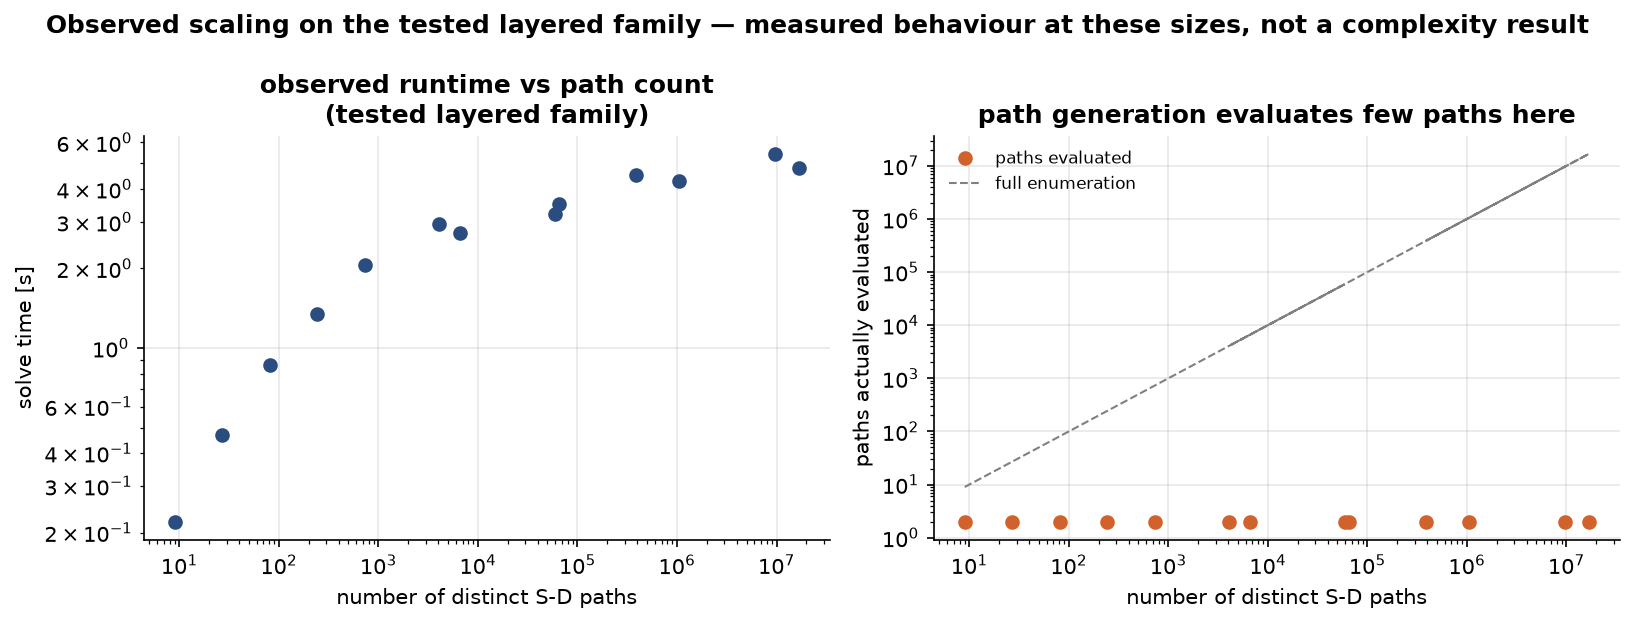
\includegraphics[width=\textwidth]{figs/E7_scaling.png}
\caption{Left: solve time barely grows as the number of possible routes
grows across seven orders of magnitude. Right: the number of routes
actually examined stays at two, regardless of how many exist, while full
enumeration (dashed line) would grow with the graph. \emph{Source:
generated by the accompanying solver code (\texttt{experiments.py},
experiment E7).}}
\label{fig:scaling}
\end{figure}

What does grow with graph size is the difficulty of \emph{proving} the
answer, not the answer itself. The proof-gap column in
Table~\ref{tab:e7} is below $10^{-9}$ up to 18 checkpoints, but on the
largest graphs (48--50 checkpoints) the lower bound has not finished
closing within our 200-iteration limit, leaving a gap of up to
$2.1\times10^{-3}$. In particular, the headline $1.68\times10^7$-route
instance is \emph{not} certified: its outer gap is $2.1\times10^{-3}$, so
we can say the solver recovers the known closed-form value there while
evaluating only two routes, but we cannot say it proves that value
optimal. The \emph{value} in those rows is exact to floating-point
precision (see the closed-form comparison in Table~\ref{tab:e7}); the
\emph{proof} that it is optimal is incomplete.
This is a known property of Kelley's method, which can converge slowly in
high dimension, with complexity depending on problem geometry and
assumptions \citep{nesterov2018}; a more advanced master problem (a
proximal-bundle or level-set method) would likely fix this and is a clear
next step.

\subsection{Effect of contest intensity}

Table~\ref{tab:e8} and Figure~\ref{fig:intensity} vary $m$ from $0.25$ to
$3$. Only the columns with $m\le1$ are certified optima $V^{\star}$; by
Proposition~\ref{prop:m-gt-1} the problem need not be convex for $m>1$,
so the entries there are the objective value of the allocation the solver
returns -- a candidate, with no guarantee that it is globally optimal. We
refer to them as \emph{reported objective values} rather than $V^{\star}$.

On the plain 4-node chain the reported value is exactly $0.0625$ for
\emph{every} $m$ tested, and here we can say more than "the solver
reports it": with equal budgets and only one route, symmetry forces
$x_i=y_i$ at every node regardless of $m$, so $p_i=\tfrac12$ and the
value is $(1/2)^4$ analytically, for all $m$. This row is therefore
exact even where the certificate does not apply. Contest intensity only
matters when one side can concentrate its resources and the other cannot.

On the grid, the reported value rises from $0.118$ at $m=0.25$ to
$0.940$ at $m=3$. The defender must spread across many parallel routes
while the evader can concentrate on one; a higher $m$ rewards
concentration, so raising contest intensity there favours the evader.
For $m\le1$ this is a statement about certified optima; for $m>1$ it
describes the solver's returned allocations, and we do not claim it as a
statement about the true game value.

\begin{table}[htbp]
\centering
\caption{Effect of contest intensity $m$ ($\XA=\XB=10$). Entries for
$m\le1$ are certified optima $V^{\star}$. Entries for $m>1$ are reported
objective values of the returned allocation and carry no optimality
guarantee (Proposition~\ref{prop:m-gt-1}); the chain row is nonetheless
exact for all $m$ by the symmetry argument in the text.}
\label{tab:e8}
\small
\begin{tabular}{lccccccc}
\toprule
 & \multicolumn{4}{c}{certified optimum $V^{\star}$} & \multicolumn{3}{c}{reported objective (not proven)}\\
\cmidrule(lr){2-5}\cmidrule(lr){6-8}
graph & $m=0.25$ & $m=0.5$ & $m=0.75$ & $m=1$ & $m=1.5$ & $m=2$ & $m=3$\\
\midrule
chain (4 nodes)  & 0.0625 & 0.0625 & 0.0625 & 0.0625 & 0.0625 & 0.0625 & 0.0625\\
3 parallel chains & 0.1835 & 0.2548 & 0.3358 & 0.4219 & 0.5898 & 0.7290 & 0.8966\\
grid $4\times4$   & 0.1177 & 0.1975 & 0.2979 & 0.4096 & 0.6243 & 0.7847 & 0.9399\\
\bottomrule
\end{tabular}
\end{table}

\begin{figure}[htbp]
\centering
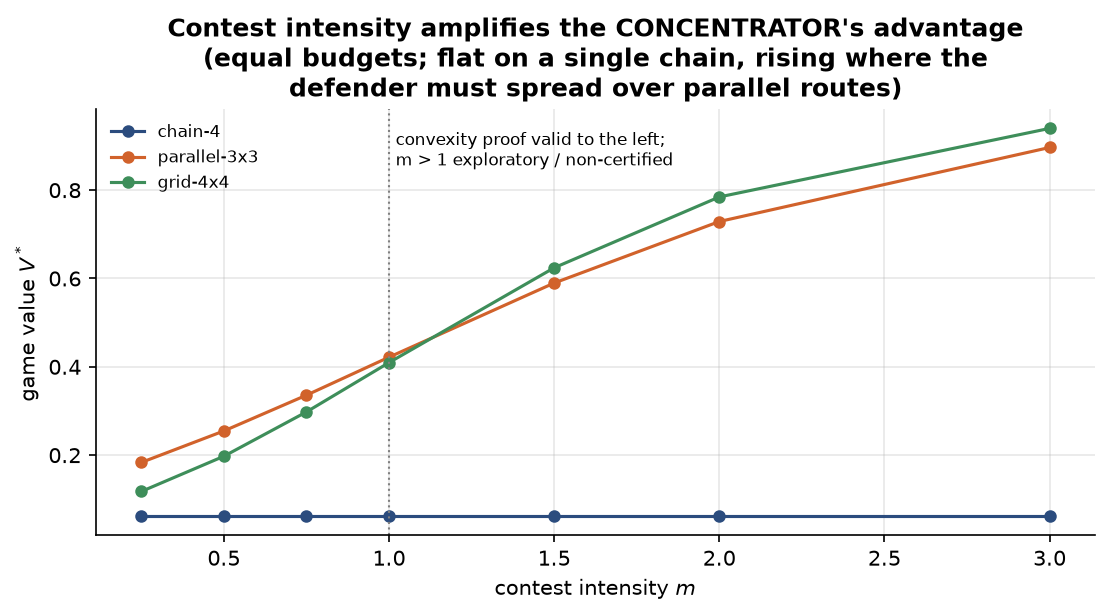
\includegraphics[width=0.72\textwidth]{figs/E8_intensity.png}
\caption{Defender objective against contest intensity $m$; certified as
$V^{\star}$ only to the left of the vertical line. The vertical
line marks the boundary of the convexity proof. The chain is flat because
equal budgets on a single route always give a $50/50$ contest regardless
of $m$; the grid and parallel-route graphs rise sharply because the
evader can concentrate its effort while the defender cannot.
\emph{Source: generated by the accompanying solver code
(\texttt{experiments.py}, experiment E8).}}
\label{fig:intensity}
\end{figure}

\subsection{Different graph shapes at a glance}
\label{sec:results-gallery}

Figure~\ref{fig:gallery} shows the optimal defence on nine different
graphs side by side, including one with a directed cycle -- the method
does not require the graph to be acyclic, since only simple (non-repeating)
routes matter to the evader. A few patterns are visible directly in the
picture. On the unequal-branches graph, the single-node branch gets about
20 times as much defence per node as the four-node branch, for the reason
given in Section~\ref{sec:methods-inner}. On the random graph, most of
the budget concentrates on just two nodes that together form a cut,
leaving several nodes at essentially zero -- the sparse-support pattern
predicted by Proposition~\ref{prop:cut}, and here it happens to coincide
with the minimum cut, though Section~\ref{sec:results-baselines} shows
this coincidence does not hold in general.

\begin{figure}[htbp]
\centering
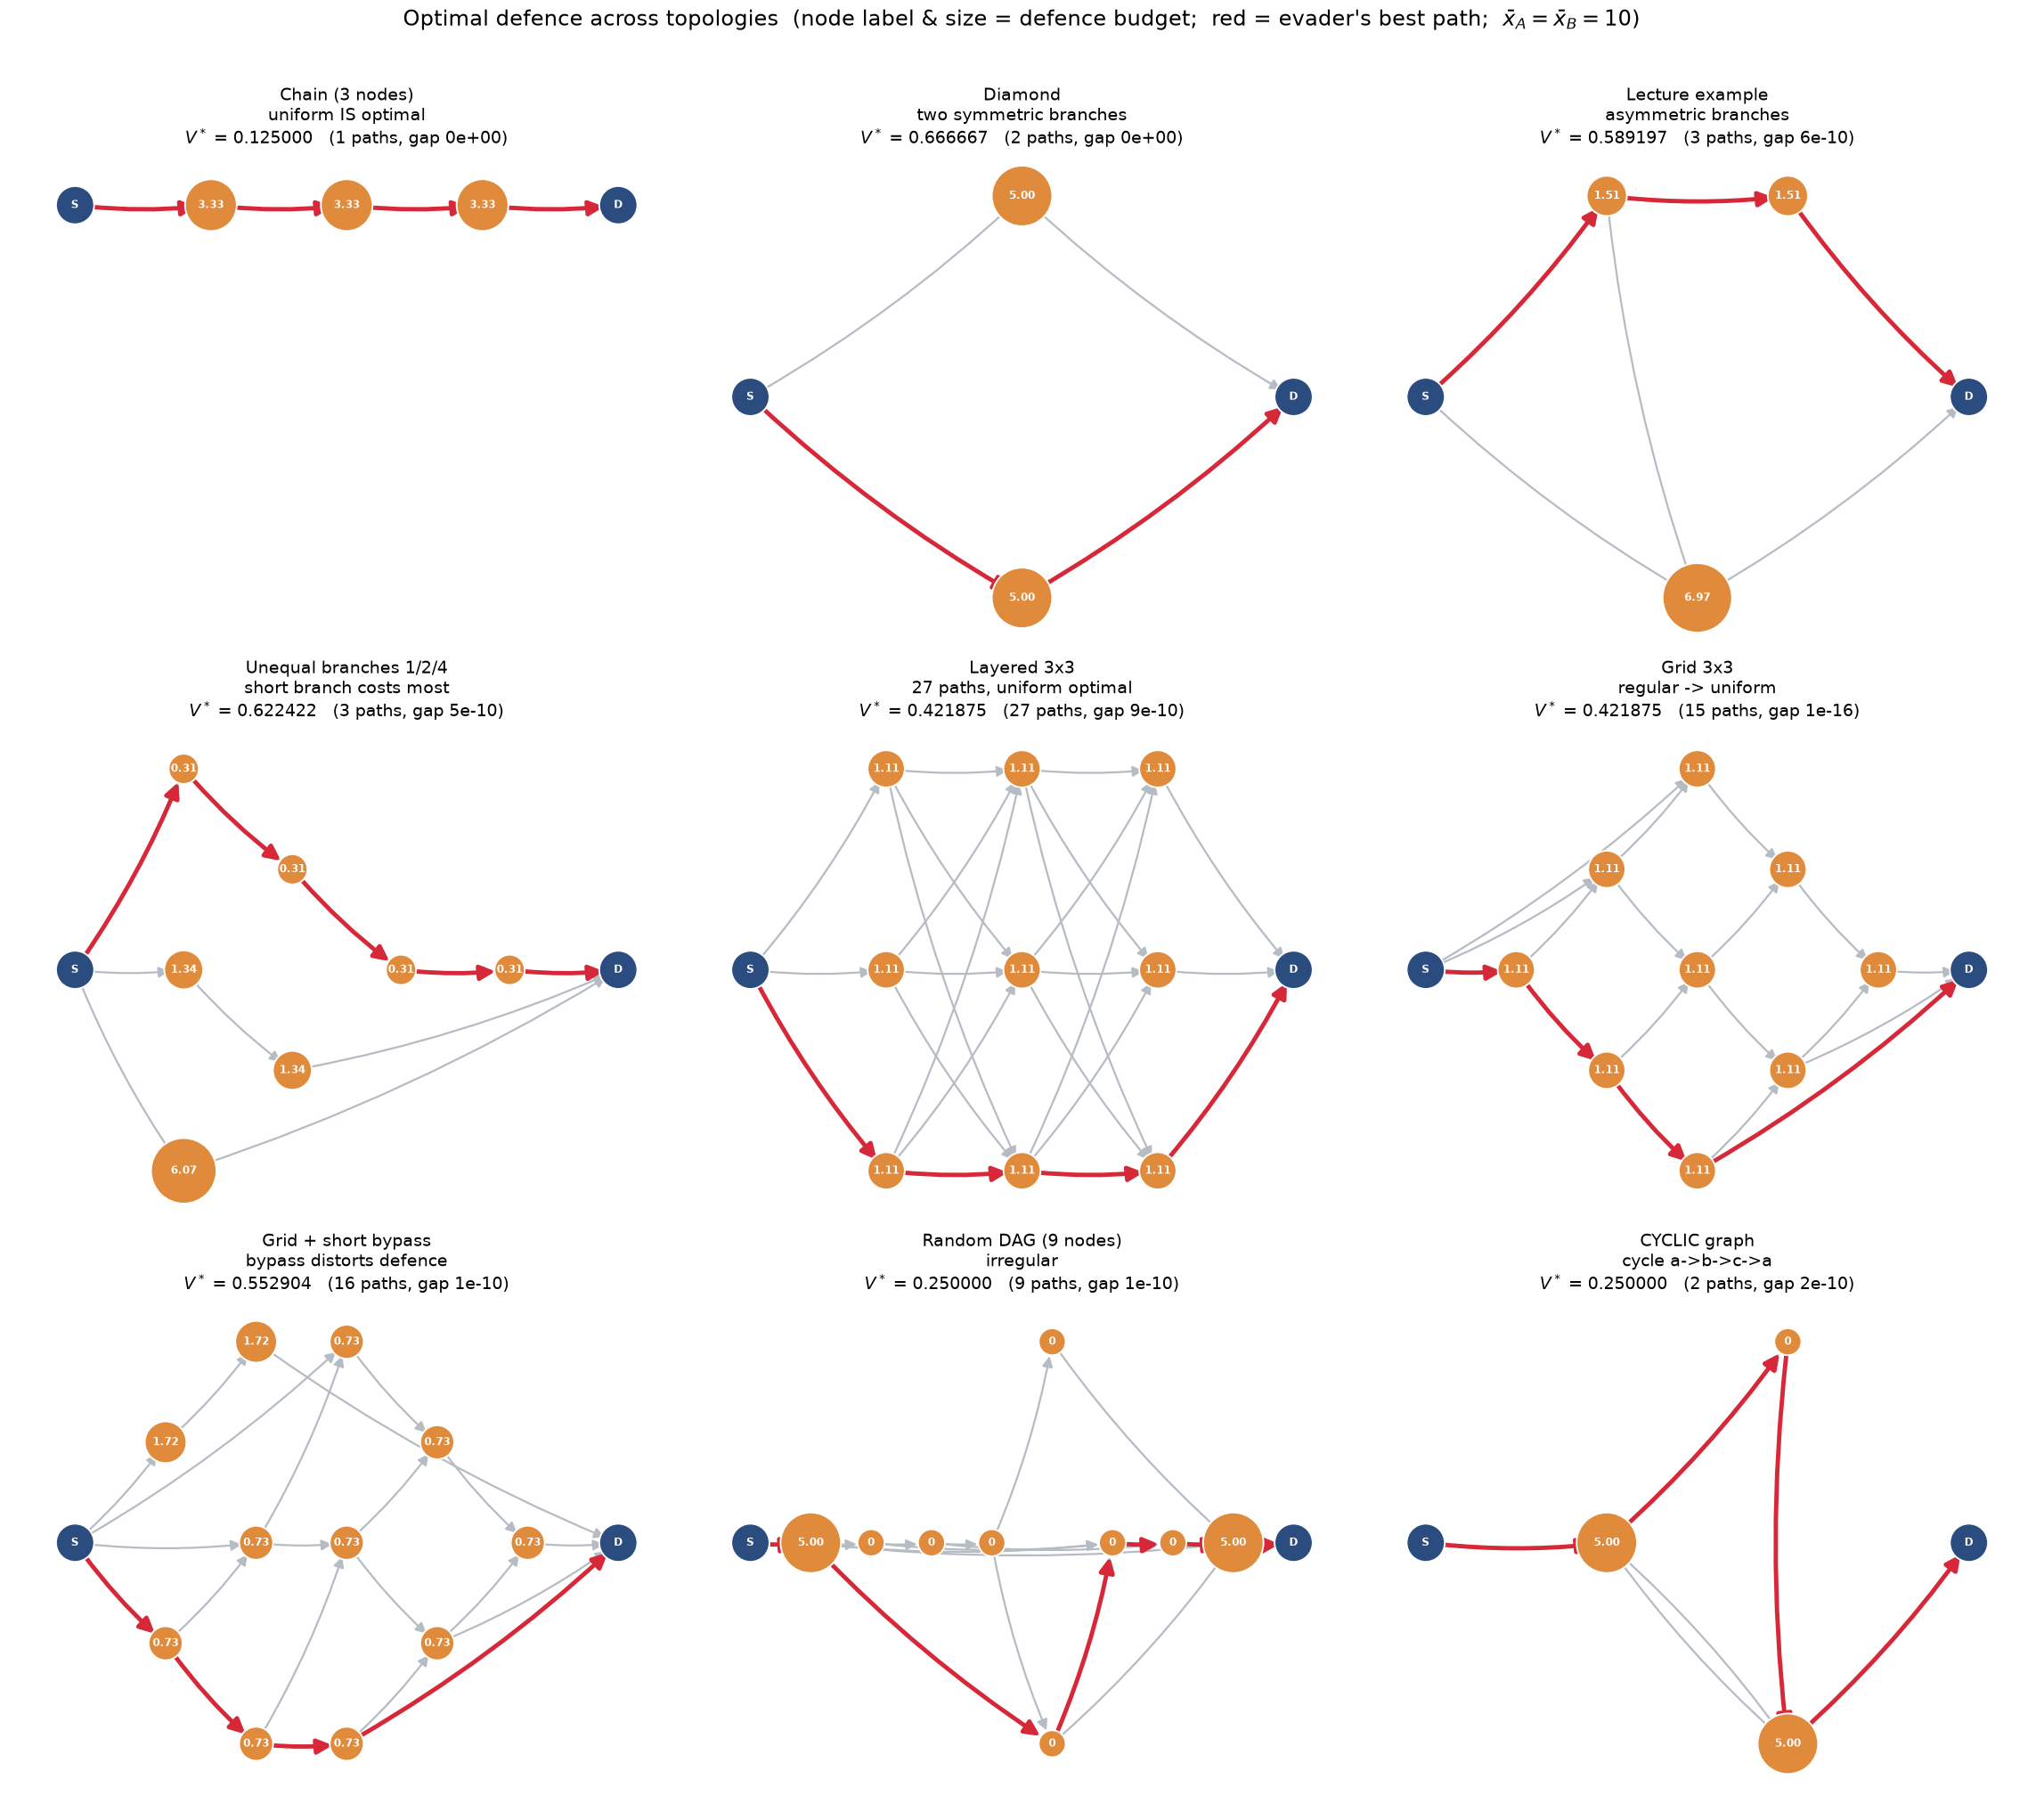
\includegraphics[width=\textwidth]{figs/GALLERY.png}
\caption{Optimal defence on nine graphs. Node size and label give the
defence budget at that node; the red path is the route the evader
actually chooses against that defence. The bottom-right graph contains a
directed cycle, confirming the method is not restricted to acyclic
graphs. \emph{Source: generated by the accompanying solver code
(\texttt{gallery.py}).}}
\label{fig:gallery}
\end{figure}

\subsection{Summary of the computational findings}
\begin{enumerate}[leftmargin=2em,itemsep=0.2em]
\item The solver matches four independently derived closed forms to
  $5.6\times10^{-12}$, and is never beaten by brute-force search.
\item The number of possible routes is not what makes an instance hard:
  the route oracle evaluates two routes whether there are nine or
  $1.68\times10^7$ of them, and graphs with very different route counts
  can have identical values.
\item Spreading the defence budget evenly is provably optimal for the
  symmetric families analysed here (chains, identical parallel chains,
  complete layered graphs) and up to $330\%$ worse than optimal on
  irregular graphs.
\item Defending only the most "central" node can fail completely,
  letting the evader through with certainty.
\item The optimality proof closes to machine precision on graphs up to
  about 20 checkpoints, but not always within our iteration limit on the
  largest graphs tested (48--50 checkpoints), even though the numerical
  answer itself remains accurate.
\end{enumerate}

%==============================================================================
\section{Discussion}
\label{sec:discussion}

\subsection{What the results mean}

The main practical message is that intuition is not a reliable guide to
network defence, even when the intuition sounds reasonable. "Spread the
budget evenly" and "protect the choke point" are both defensible-sounding
rules, and both can be far from optimal, sometimes catastrophically so.
The reason, in both cases, is the same: neither rule accounts for how
route \emph{length} interacts with the contest at each node. A short
route needs much more defence per node than a long one, because a long
route already punishes the evader through repeated multiplication
(Equation~\ref{eq:symmetric}). A rule that ignores this -- like spreading
the budget by node count, or by how many routes pass through a node --
will systematically under-defend short routes and over-defend long ones.

The value of a certified method, rather than a heuristic one, is that it
tells you not just an allocation but how far from optimal any other
allocation is. Table~\ref{tab:e5} would not be a meaningful table at all
if we could not first solve for the true optimum.

\subsection{Where the method stops applying}

We list the boundaries of the method plainly, since several of them
matter for how the results should be used.

\begin{description}[leftmargin=1.4em,style=nextline]
\item[Contest intensity above 1 is not certified.] Convexity provably
  fails there (Proposition~\ref{prop:m-gt-1}); the solver still produces
  numbers, but with no proof attached. Whether any solution concept --
  pure or mixed -- can be characterised in that regime is left open.
\item[The game is sequential, not simultaneous.] The defender commits
  first. A simultaneous version would generally require mixed strategies
  over routes, which is the setting studied by \citet{nguyen2023}.
\item[No proven speed of convergence.] We show empirically that the
  method converges (Section~\ref{sec:results-scaling}), but we do not
  prove how fast. Kelley's method can converge slowly, and its complexity
  depends on the geometry and assumptions of the problem
  \citep{nesterov2018}. The partial strict convexity of
  Proposition~\ref{prop:partial-strict} is a natural starting point for
  deriving a rate, which we have not attempted.
\item[The comparison set is generic rules, not competing methods.] We
  compare against simple, commonly suggested rules -- even split, minimum
  cut, route count, centrality, greedy -- not against a re-implementation
  of the evolutionary method in \citet{ramirez2011} or the integer
  program in \citet{nguyen2023} run on the same graphs. A more complete
  study would include that direct comparison.
  % TODO(author): this is the single most valuable additional experiment
  % if more time is available before submission.
\item[Nodes are assumed independent.] The payoff is a product of
  per-node survival probabilities, which assumes detection events at
  different checkpoints do not influence each other. Real checkpoints
  often share information or infrastructure, which would break this
  assumption.
\item[Only node contests are modelled.] Contests on edges (rather than
  nodes) would need each edge turned into a node, which is a
  straightforward change but is not implemented here.
\item[The route oracle is certified but not guaranteed fast.] In the
  worst case it can still degrade to checking every route, since the
  underlying problem is NP-hard \citep{nguyen2023}.
\item[The uniqueness proof deserves an independent reading.] Uniqueness
  is proved (Lemma~\ref{lem:active-cover},
  Proposition~\ref{prop:uniqueness}) for $0<m\le1$ when $V^{\star}<1$,
  via an active-cover argument rather than strict convexity of $G$, which
  genuinely fails. An earlier version of this work contained a different
  and \emph{incorrect} uniqueness proof. Automated testing can refute a
  proof but never confirm one, so this result -- like the convexity
  theorem itself -- should be checked independently before it is relied
  on.
\item[Novelty has not been independently confirmed.] The literature
  search behind Section~\ref{sec:litreview} found no exact match, but it
  is a keyword search, not a systematic review, and should be checked
  against a supervisor's knowledge of the area before any claim of
  novelty is made in a submission.
\end{description}

%==============================================================================
\section{Conclusion}
\label{sec:conclusion}

A network defender with a fixed budget, facing an evader who picks both a
route and how hard to try at each checkpoint on it, faces a problem that
looks intractable at first: an exponential number of possible routes, and
an objective that is not obviously convex or concave. We showed that,
written in the right coordinates, the problem is convex whenever the
contest intensity does not exceed 1, which makes a certified global
optimum reachable, and we gave an explicit graph on which convexity fails
above that threshold. Whether the optimal allocation is also unique
remains open: we prove strict convexity only in the coordinates of the
route attaining the maximum, which is not enough to rule out a flat set
of minimisers, though we did not observe one numerically.

Algorithmically, a Lagrangian relaxation that is additive across nodes
turns the search over possibly millions of routes into a single
shortest-path computation, with a rule that proves when the search can
stop; the outer allocation problem then yields to cutting planes with
two-sided bounds. On graphs with more than sixteen million possible
routes, the route oracle recovers the known value while examining only
two routes -- though on those largest instances the outer certificate
does not close within our iteration limit, so the value is accurate
without being proved optimal.

The applied conclusion is a caution against intuition. Spreading a
defence budget evenly, or protecting the most obviously important nodes,
are not safe defaults. The even split is provably right on the symmetric
families we analyse, and can be badly wrong the moment a graph is not
symmetric, which most real networks are not.

The clearest next steps are: settling the uniqueness question; a faster
master problem to close the optimality proof on large graphs; a
characterisation of what happens above contest intensity 1; a version of
the game where both players move at the same time, which would likely
require mixed strategies over routes; and a head-to-head comparison
against the solution methods used in the two papers this work is closest
to.

%==============================================================================
\section*{Acknowledgements}
% TODO(author): add acknowledgements and funding information here.

\subsection*{A note on the use of AI tools}
% TODO(author): most venues now require a disclosure of this kind; check
% your target venue's exact wording and adjust before submission.
Parts of the software implementation, the literature search, and the
drafting of this manuscript were produced with the assistance of a large
language model. All mathematical statements were checked by hand by the
authors, and every numerical result reported here was produced by the
accompanying source code and can be reproduced from it directly.

\subsection*{Data and code availability}
% TODO(author): add a repository link or archival DOI.
All source code, the automated test suite, and the scripts that generate
every table and figure in this paper are available at
\texttt{[repository link]}.

%==============================================================================
\begin{thebibliography}{99}

\bibitem[Bloch et al.(2023)]{bloch2023}
F.~Bloch, K.~Chatterjee, and B.~Dutta.
\newblock Attack and interception in networks.
\newblock \emph{Theoretical Economics}, 18(4):1511--1546, 2023.

\bibitem[Kovenock and Roberson(2018)]{kovenock2018}
D.~Kovenock and B.~Roberson.
\newblock The optimal defense of networks of targets.
\newblock \emph{Economic Inquiry}, 56(4):2195--2211, 2018.

\bibitem[Oruganti et al.(2023)]{oruganti2023}
P.~S. Oruganti, P.~Naghizadeh, and Q.~Ahmed.
\newblock The impact of network design interventions on the security of
  interdependent systems.
\newblock arXiv:2302.05411, 2023.

\bibitem[Bozbay and Vesperoni(2018)]{bozbay2018}
I.~Bozbay and A.~Vesperoni.
\newblock A contest success function for networks.
\newblock \emph{Journal of Economic Behavior \& Organization}, 150:404--422, 2018.

\bibitem[Danskin(1967)]{danskin1967}
J.~M. Danskin.
\newblock \emph{The Theory of Max-Min and its Application to Weapons Allocation Problems}.
\newblock Springer, Berlin, 1967.

\bibitem[Hausken(2008)]{hausken2008}
K.~Hausken.
\newblock Strategic defense and attack for series and parallel reliability systems.
\newblock \emph{European Journal of Operational Research}, 186(2):856--881, 2008.

\bibitem[Iliaev et al.(2023)]{iliaev2023}
D.~Iliaev, S.~Oren, and E.~Segev.
\newblock A Tullock-contest-based approach for cyber security investments.
\newblock \emph{Annals of Operations Research}, 320(1):61--84, 2023.

\bibitem[Israeli and Wood(2002)]{israeli2002}
E.~Israeli and R.~K. Wood.
\newblock Shortest-path network interdiction.
\newblock \emph{Networks}, 40(2):97--111, 2002.

\bibitem[Kelley(1960)]{kelley1960}
J.~E. Kelley.
\newblock The cutting-plane method for solving convex programs.
\newblock \emph{Journal of the Society for Industrial and Applied Mathematics}, 8(4):703--712, 1960.

\bibitem[Nesterov(2018)]{nesterov2018}
Y.~Nesterov.
\newblock \emph{Lectures on Convex Optimization}.
\newblock Springer, 2nd edition, 2018.

\bibitem[Nguyen et al.(2023)]{nguyen2023}
D.~H. Nguyen, Y.~Song, and J.~C. Smith.
\newblock A two-stage network interdiction-monitoring game.
\newblock \emph{Networks}, 81(3):334--358, 2023.

\bibitem[Ramirez-Marquez et al.(2011)]{ramirez2011}
J.~E. Ramirez-Marquez, C.~M. Rocco, and G.~Levitin.
\newblock Optimal network protection against diverse interdictor strategies.
\newblock \emph{Reliability Engineering \& System Safety}, 96(3):374--382, 2011.

\bibitem[Skaperdas(1996)]{skaperdas1996}
S.~Skaperdas.
\newblock Contest success functions.
\newblock \emph{Economic Theory}, 7(2):283--290, 1996.

\bibitem[Smith and Song(2020)]{smith2020}
J.~C. Smith and Y.~Song.
\newblock A survey of network interdiction models and algorithms.
\newblock \emph{European Journal of Operational Research}, 283(3):797--811, 2020.

\bibitem[Tullock(1980)]{tullock1980}
G.~Tullock.
\newblock Efficient rent seeking.
\newblock In J.~M. Buchanan, R.~D. Tollison, and G.~Tullock, editors, \emph{Toward a Theory of the Rent-Seeking Society}, pages 97--112. Texas A\&M University Press, 1980.

\bibitem[Washburn and Wood(1995)]{washburn1995}
A.~Washburn and K.~Wood.
\newblock Two-person zero-sum games for network interdiction.
\newblock \emph{Operations Research}, 43(2):243--251, 1995.

\bibitem[Yen(1971)]{yen1971}
J.~Y. Yen.
\newblock Finding the $k$ shortest loopless paths in a network.
\newblock \emph{Management Science}, 17(11):712--716, 1971.

\end{thebibliography}

\end{document}
